\chapter{Firmas espectrales}
Esta clase contien dos objetivos: en principio familiarizarse con el entorno gráfico del \emph{Sentinel Aplication Toolbox (SNAP)} y además comprender el concepto de firma espectral estudiando sus valores dentro de la imagen.

\section{Interfaz gráfica del SNAP}

Descomprima los archivos decargados que se denominan \path{material.tar.gz}. Abra el programa SNAP, allí encontrará la interfaz gráfica del usuario (Figura \ref{fig:int})

\begin{figure}[h!]
    \centering
    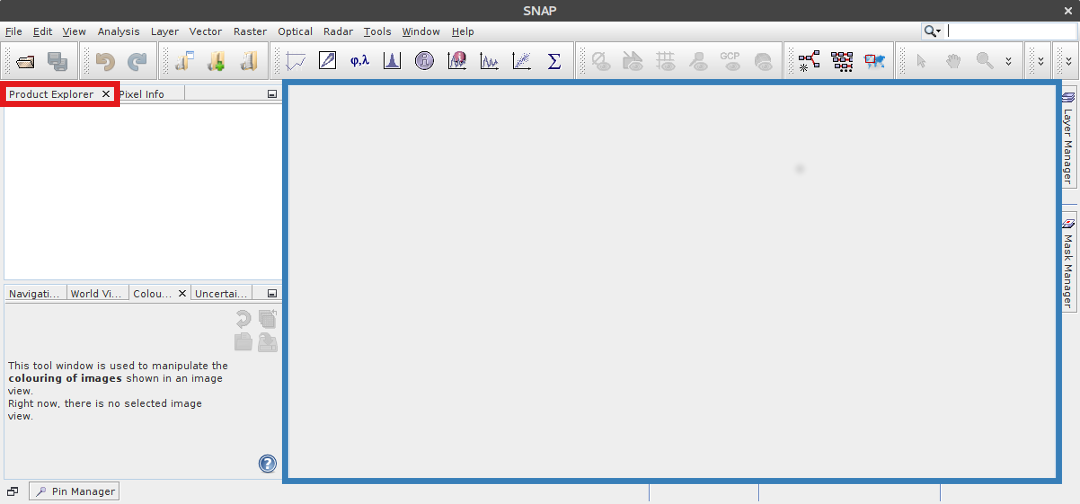
\includegraphics[scale=1.1]{fig:int.png}
    \caption{Interfáz gráfica del usuario. El árbol de capas y el área de visualización del programa.}
    \label{fig:int}
\end{figure}

En el menú principal, seleccione \emph{Open product...} o presione [BOTON ABRIR] y dentro de la carpeta \path{material/raster_data}, seleccione \path{S2A_MSIL2A_20170720.dim}.

La cobertura que aparecerá en el árbol de capas es más completa que la típica cobertura raster que se encuentra en la mayoría de los software.NO LO PONDRIA

Haga doble click sobre el nombre y se desplegará un árbol que incluye las siguientes opciones:
\dirtree{%
    .1 [1] S2\_MSIL2A\_20170702.
    .2 Metadaata.
    .2 Index Codings.
    .2 Vector Data.
    .2 Bands.
    .2 Masks.
}

De esta cobertura se destaca:

\begin{itemize}
    \item \emph{[1] S2\_MSIL2A\_20170702}: El número de elemento entre corchetes y el nombre de la imagen.
    \item \emph{Metadata}: Los metadatos asociados a la imagen y su historial de procesamiento.
    \item \emph{Index Codings}: Los valores de referencia de como interpretar dentro de la imagen y las máscaras distintos valores.
    \item \emph{Vector data}: Las capas vectoriales asociadas a la imagen.
    \item \emph{Bands}: Las bandas de la imagen y las operaciones de álgebra entre bandas. Haciendo doble click puede mostrarlas en el visualizador.
    \item \emph{Masks}: Las máscaras que sean incluidas en la imagen o las que crearán.
\end{itemize}


\begin{que}
    ¿Cuantas bandas encuentra dentro del archivo? ¿A qué longitudes de onda corresponden? ¿En qué zonas del espectro está el mayor número de bandas?
\end{que}

\section{Combinaciones espectrales}

En \emph{Product Explorer} haga click derecho sobre el nombre y seleccione \emph{Open RGB image windows.}. Se desplegará una nueva ventana (Figura \ref{fig:RGB}) que le permitirá elegir la combinación de bandas.

\begin{figure}[h!]
    \centering
    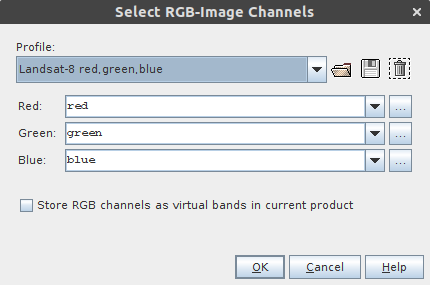
\includegraphics[scale=0.7]{fig:RGB.png}
    \caption{Ventana de combinación de bandas. Puede eligir una banda para cada canal del monitor ()\emph{Red, Green, Blue}) o puede optarpor una preseleccionada del menú \emph{Profile}}
    \label{fig:RGB}
\end{figure}

Por defecto elegirá la combinación que utiliza las bandas 4, 3 y 2 de Sentinel 2 y la desplegará haciendo click en OK (Figura \ref{fig:RVA}).

\begin{figure}[h!]
    \centering
    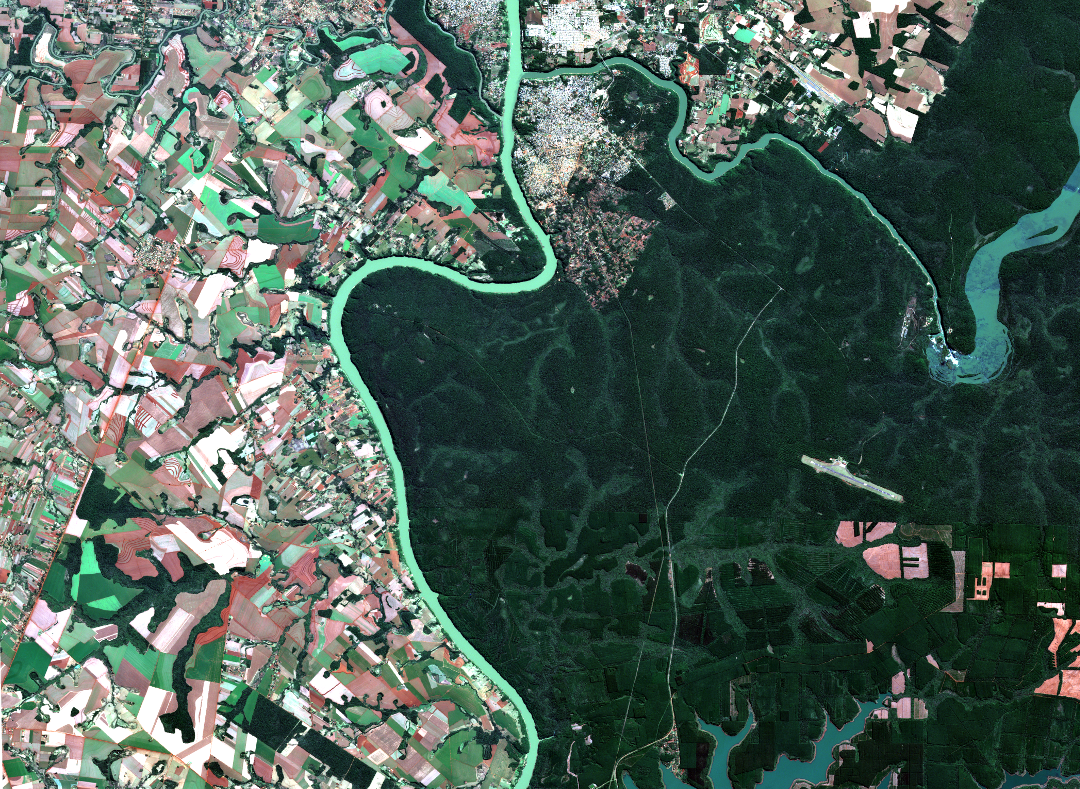
\includegraphics[scale=0.5]{fig:RVA.png}
    \caption{Imagen en combinación de colores de color real.}
    \label{fig:RVA}
\end{figure}

\begin{que}
    ¿A qué longitudes de onda pertenecen cada una de estas bandas? ¿Con qué colores las identificamos?
\end{que}

Explore la imagen utilizando las herramientas de navegación y zoom (Figura \ref{fig:NAV})

\begin{figure}[h!]
    \centering
    
\includegraphics[scale=0.5]{fig:NAV.png}
    \caption{Herramientass de navegación.}
    \label{fig:NAV}
\end{figure}



\begin{que}
    ¿Observa diferencias en los colores de los distintos cuerpos de agua? ¿Y en los colores de la selva y las forestaciones? ¿Que le dice la diferencia observada sobre la firma espectral de los distintos cuerpos de agua? ¿Será posible separar espectralmente las forestaciones de la selva utilizando unicamente la zona visible del espectro electromagnetico?
\end{que}

Seleccione ahora la combinacion de color RGB \emph{Sentinel 2 MSI False-color Infrarred} que incluye a una banda del infrarrojo cercano y dos del visible (Figura \ref{fig:NRG}). Explore la imagen desplegada en esta combinación de color.

\begin{figure}[h!]
    \centering
    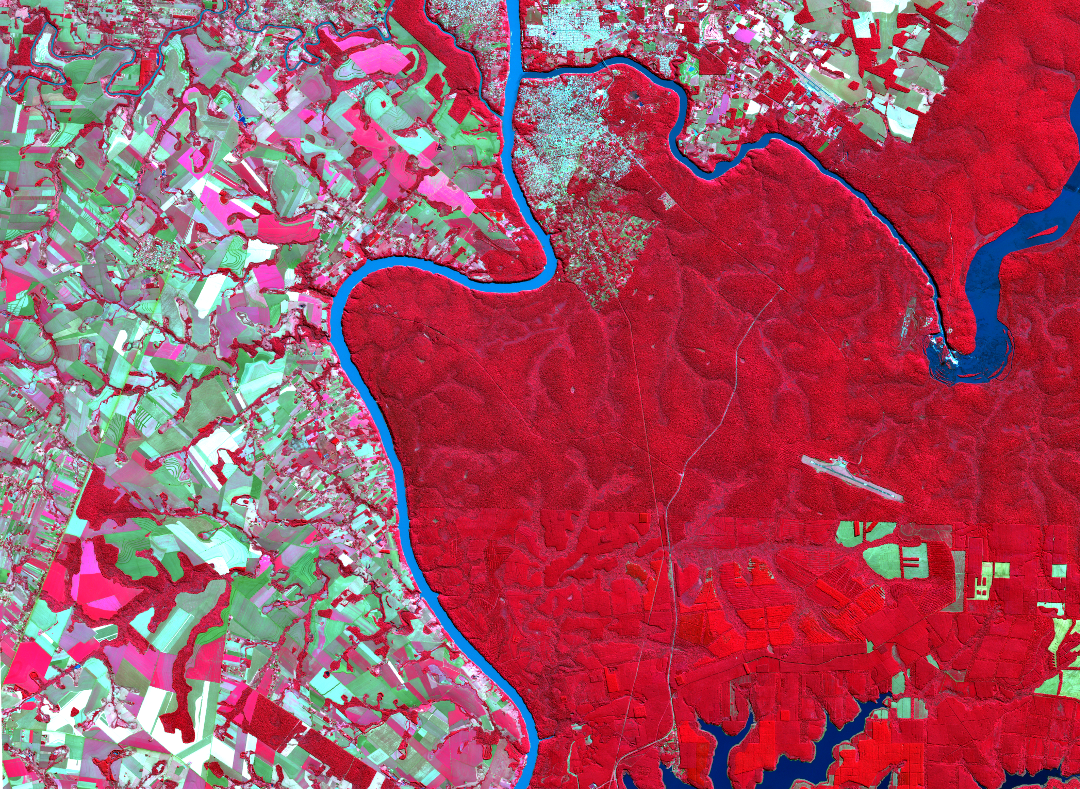
\includegraphics[scale=0.5]{fig:NRG.png}
    \caption{Imagen en combinación de colores infrarrojo color.}
    \label{fig:NRG}
\end{figure}

\begin{que}
    ¿Observa diferencias en los colores de los distintos cuerpos de agua? ¿Pueded distinguir más o menos detalles dentro de los mismos que con la combinación de color real? ¿Y en los colores de la selva y las forestaciones? ¿Será posible separar espectralmente las forestaciones de la selva utilizando unicamente la zona del espectro visible del visible y el infrarrojo cercano? ¿Considerando la relación entre la reflectancia en el NIR y los parametros biofísicos, que pueded predecir sobre el porcentaje de cobertura de la selva y las forestaciones?
\end{que}

Seleccione ahora la combinacion de color RGB \emph{Sentinel 2 MSI Healthy Vegetation} que incluye a una banda del infrarrojo cercano, una del infrarrojo medio y una del visible (Figura \ref{fig:SNR}). Explore la imagen desplegada en esta combinación de color.

\begin{figure}[h!]
    \centering
    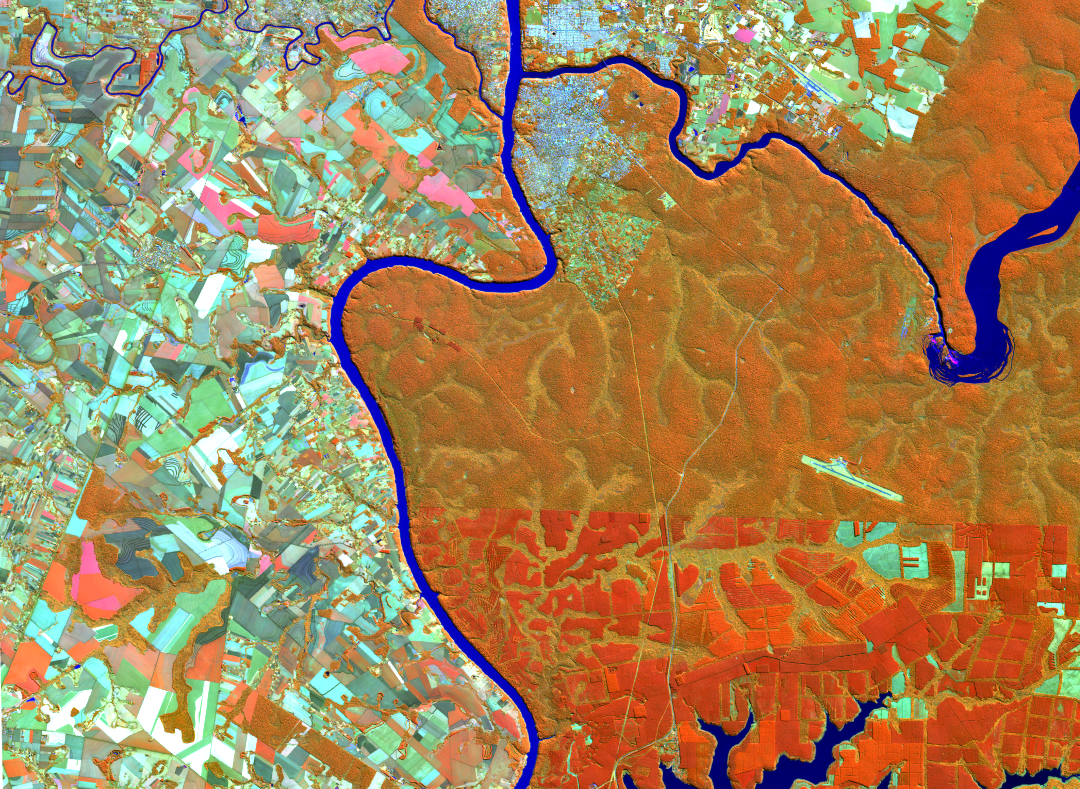
\includegraphics[scale=0.5]{fig:SNR.png}
    \caption{Imagen en combinación de colores falso color compuesto.}
    \label{fig:SNR}
\end{figure}


\begin{que}
    ¿Es posible separar a las forestaciones de la selva en ésta combinación de bandas? ¿Cuál es la caracteristica biofísica que  manifiesta mayor cambio entre la selva y las forestaciones? ¿Es posible distinguir grandes diferencias entre los cuerpos de agua en esta combinación de bandas?
\end{que}

\begin{que}
    ¿Que combinación de bandas le aporta más información sobre la vegetación? Explique desde el punto de vista de la firma espectral de la vegetación,  según sus variaciones en cada zona y teniendo en cuenta las propiedades biofísicas. ¿Qué combinación de bandas le aporta más información sobre los cuerpos de agua?
\end{que}

\section{Firmas espectrales}

En el menú principal \emph{Optical} seleccione la opción \emph{Spectrum view}. Esta herramienta permite extraer los valores de un píxel en función de la longitud de onda, mostrarlo como gráfico de lineas (Figura \ref{fig:sps}) o guardados en un archivo de texto.

\begin{figure}[h!]
    \centering
    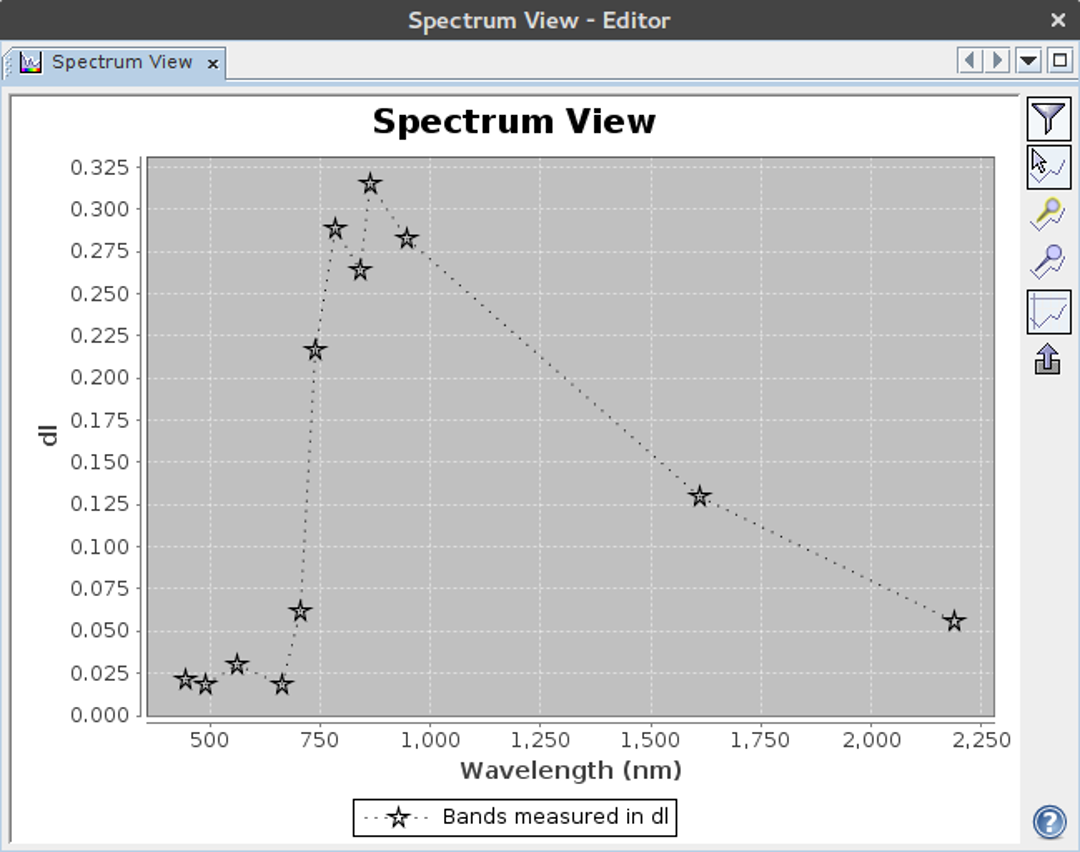
\includegraphics[scale=0.7]{fig:sps.png}
    \caption{Herraamienta \emph{Spectrum view} que permite mostrar lass firmas espectrales de distintos píxeles de la imagen.YO PONDRIA EL  NOMBRE DE LOS BOTONES LATERALES}
    \label{fig:sps}
\end{figure}

Despliegue la imagen \path{S2A_MSIL2A_20170720.dim} en una combinación de bandas conveniente para identificar distintas coberturas de vegetación Y observe sus firmas espectrales.

\begin{que}
    ¿Cómo es la la firma espectral de la vegetación para las zonas de la selva que parecen hallarse más altas? %ver lo de alto
    ¿Y para las zonas de forestación? ¿Qué pasa con la firma espectral de la ciudad de Puerto Iguazu?
\end{que}

Es posiblemostrar varias firmas espectrales en simultaneo utilizando marcas (PIN). Para hacerlo seleccione la herramienta \emph{Pin placement tool}  de la barra de herramienta %icono
 y haga click sobre la imagen (Figura \ref{fig:pin}).

\begin{figure}[h!]
    \centering
    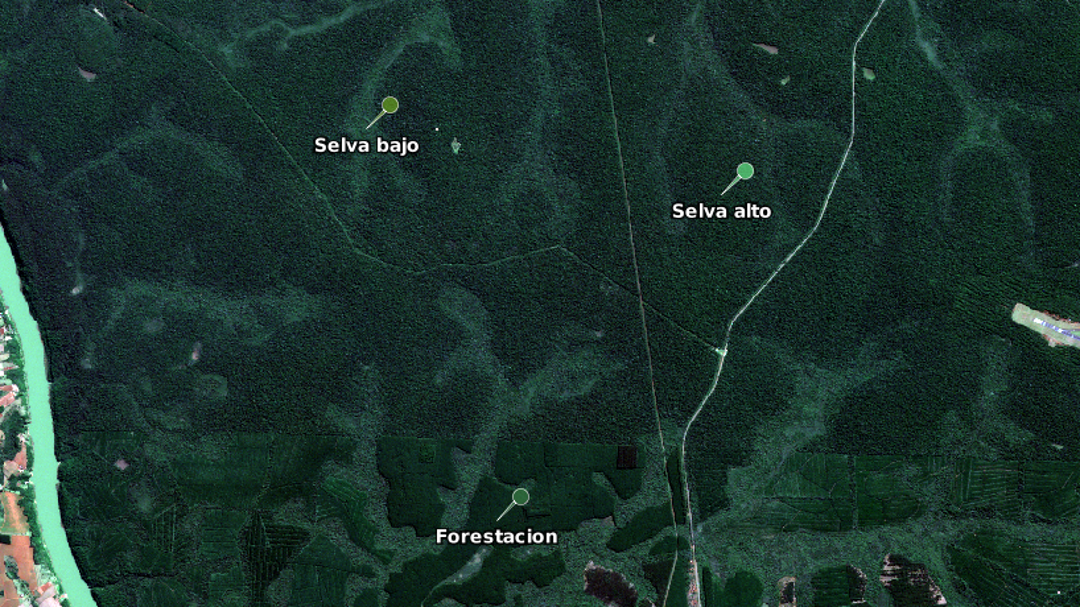
\includegraphics[scale=0.7]{fig:pin.png}
    \caption{Pin sobre un píxel en la imagen.}
    \label{fig:pin}
\end{figure}

Utilice la herramienta \emph{Pin placement tool} para generar pines en distintas zonas de la imagen. Incluya al menos dos zonas de la selva cualitativamente ditintas, una zona de forestación y al menos un pin en el embalce Urugua-I, uno en el Rio Parana y otro en el Iguazu.

Haciendo click en \emph{Pin manager} se desplegará una nueva ventana con sus propiedades. Puede observar el pixel sobre el que se encuentra, su latitud y longitud, el color que se mostraŕa y la etiqueta \footnote{Label}. Asgine a cada pin una etiqueta y color diferenciado (Figura \ref{fig:pmg}).

\begin{figure}[h!]
    \centering
    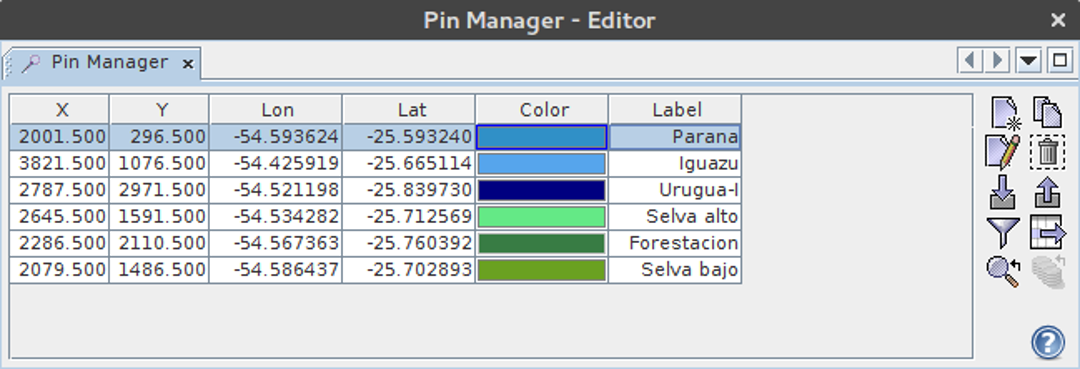
\includegraphics[scale=0.7]{fig:pmg}
    \caption{Ping manager}
    \label{fig:pmg}
\end{figure}

Con la herramienta \emph{Spectrum view} puede mmostrar todas las firmas espectrales al mismo tiempo \emph{Show spectra for all pins}, o por separado \emph{Show spectra for selected pins} (Figura \ref{fig:spn}).

\begin{figure}[h!]
    \centering
    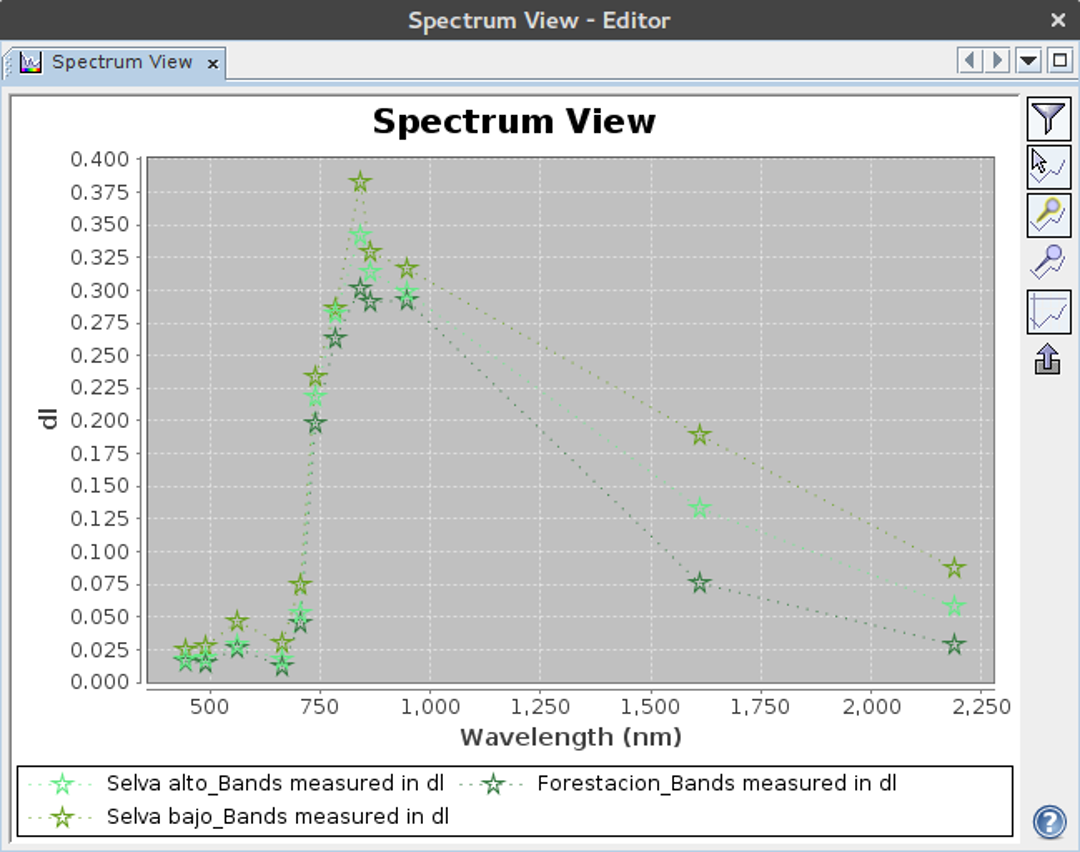
\includegraphics[scale=0.7]{fig:spn.png}
    \caption{Firmas espectrles de los pines seleccionados}
    \label{fig:spn}
\end{figure}

Haciendo click derecho sobre la firma espectral se despliega una lista de opciones. Entre ellas \emph{Zoom in}, \emph{Zoom out} y \emph{Auto-range} para cambiar la escala del gráfico o \emph{Save as...} para guardarlo.
Con el botón \emph{Export spectra to text file} de la banda lateral puede exportar los valores de reflectancia.

Compare las firmas espectrales de las zonas de forestación y selva paranense (Figura \ref{fig:spn}).%?????

\begin{que}
    ¿En qué zonas del espectro son similares las firmas de Selva Alta %ver
    y Forestación? ¿En qué zonas del espectro son distintas las tres firmasa espectrales? ¿Qué le permite decir esto sobre el contenido de contenido de relativo de pigmentos de las tres coberturas? ¿Y sobre el contenido relativo de humedad en la vegetación? ¿Qué suposición está realizando al comparar las tres firmas de vegetación?
\end{que}

Compare las firmas espectrales del río Parana y el río Iguazu cerca de la zona donde se juntan.

\begin{que}
    ¿En que zona del espectro electromagnético son más distintass las firmas espectrales? ¿A que se debe esta diferencia? ¿Qué le dice sobre la combinación de bandas que más nos permite distinguir propiedades en los cuerpos de agua? ¿Cuál de los dos ríos parece tener mayor contenido de sedimento? ¿Por qué?
\end{que}
